%% —-----------------------------------------------------------
%% main.tex — Relatório do projeto PetCare
%% Baseado no template SBC Reviews 2025 (sbcreviews-pt.tex),
%% Licença CC BY 4.0, Sociedade Brasileira de Computação.
%%
%% COMPILAR COM XeLaTeX OU LuaLaTeX (no Overleaf: Menu -> Compiler).
%% Trechos marcados com \pendente{...} aparecem em vermelho no PDF
%% e devem ser completados pela equipe.
%% —-----------------------------------------------------------

\documentclass[portuguese]{sbcreviews-2025}%
\usepackage[misc,geometry]{ifsym}

\usepackage{aas_macros}
\usepackage[bottom]{footmisc}

\usepackage{tabularray}
\usepackage{afterpage}
\usepackage{url}
\usepackage{pifont}

% --- Pacotes adicionais deste relatório (todos padrão no TeX Live/Overleaf) ---
\usepackage{tikz}
\usetikzlibrary{positioning,arrows.meta,fit,backgrounds,calc}
\usepackage{listings}

\setcitestyle{square}

\definecolor{engtitle}{rgb}{0.5,0.5,0.5}
\definecolor{orcidlogo}{rgb}{0.37,0.48,0.13}
\definecolor{unilogo}{rgb}{0.16, 0.26, 0.58}
\definecolor{maillogo}{rgb}{0.58, 0.16, 0.26}
\definecolor{darkblue}{rgb}{0.0,0.0,0.0}
\hypersetup{colorlinks,breaklinks,
            linkcolor=darkblue,urlcolor=darkblue,
            anchorcolor=darkblue,citecolor=darkblue}

% --- Marcador de pendências (texto vermelho) ---
\definecolor{pendcolor}{rgb}{0.80,0.0,0.0}
\newcommand{\pendente}[1]{{\color{pendcolor}\textbf{[PENDENTE:}~#1\textbf{]}}}

% --- Listagens (JSON do contrato da API) ---
\lstset{
  basicstyle=\ttfamily\footnotesize,
  columns=fullflexible,
  keepspaces=true,
  breaklines=true,
  frame=single,
  framerule=0.4pt,
  xleftmargin=2pt,
  xrightmargin=2pt,
  showstringspaces=false
}

\jid{ROCS}
\jtitle{SBC Computing Reviews, 202X, XX:1}
\issn{2966-3938}
\doi{10.5753/rocs.202X.XXXXXX}
\copyrightstatement{This work is licensed under a Creative Commons Attribution 4.0 International License}
\jyear{2026}

\category{Relatório Técnico}
\title[PetCare: monitoramento de gatos com ESP32]{PetCare: sistema de monitoramento de rotina e saúde de gatos domésticos com ESP32, sensores de baixo custo e aplicação web}
\engtitle{\textcolor{engtitle}{PetCare: a domestic cat routine and health monitoring system based on the ESP32, low-cost sensors and a web application}}

%THE ORCID IS MANDATORY FOR EACH AUTHOR
\author[\pendente{Sobrenome} et al. 2026]{
\affil{\textbf{\pendente{Autor 1}}~\orcidlink{0000-0000-0000-0000}~\textcolor{blue}{\faEnvelope}~~[{\pendente{Instituição}}~|\href{mailto:autor1@exemplo.br}{~{\textit{\pendente{e-mail}}}}~]}

\affil{\textbf{\pendente{Autor 2}}~\orcidlink{0000-0000-0000-0000}~[{\pendente{Instituição}}~|\href{mailto:autor2@exemplo.br}{~{\textit{\pendente{e-mail}}}}~]}

\affil{\textbf{\pendente{Autor 3}}~\orcidlink{0000-0000-0000-0000}~[{\pendente{Instituição}}~|\href{mailto:autor3@exemplo.br}{~{\textit{\pendente{e-mail}}}}~]}
}

\begin{document}

\begin{frontmatter}

\maketitle

\begin{mail}
\pendente{Departamento/Curso, Universidade, Endereço, Cidade, Estado, CEP, Brasil.}
\end{mail}

\begin{abstract-pt}
Este relatório descreve o PetCare, um sistema de \textit{home care} para gatos domésticos desenvolvido na disciplina de \pendente{nome da disciplina de Eletrônica Analógica/Instrumentação}. Um microcontrolador ESP32 lê três tipos de sensor: um módulo de microfone de eletreto com comparador LM393, do qual se extraem características acústicas das vocalizações do gato (duração, frequência fundamental, tonalidade, taxa de cruzamentos por zero, rajadas e envelope de volume); um sonar ultrassônico LV-MaxSonar-EZ1, lido por UART, que detecta entradas e saídas da caixa de areia por variação em relação a uma distância de referência; e um sensor capacitivo de proximidade que indica presença ou ausência de água/ração na altura em que está instalado. O firmware, escrito em C sobre o ESP-IDF, inclui pareamento Wi-Fi por ponto de acesso próprio (SoftAP), persistência de configuração em memória não volátil e descoberta automática do servidor por \textit{broadcast} UDP. As leituras são enviadas a uma API REST (Node.js, Express e MongoDB), que classifica heuristicamente o tipo de vocalização, e exibidas em uma aplicação web (React) com planta baixa interativa, painel de dados e aba de saúde. O texto discute as escolhas de condicionamento de sinal e as limitações dos sensores de baixo custo empregados. \pendente{Completar com os principais resultados experimentais e conclusões após os testes.}
\end{abstract-pt}

\begin{abstract-en}
This report describes PetCare, a home care system for domestic cats. An ESP32 microcontroller reads an electret microphone module with an LM393 comparator, from which acoustic features of cat vocalizations are extracted; an LV-MaxSonar-EZ1 ultrasonic rangefinder read over UART, which detects litter box visits; and a capacitive proximity sensor that indicates the presence of water/food at its mounting height. The ESP-IDF firmware provides SoftAP Wi-Fi provisioning, non-volatile configuration storage and UDP-based server discovery. Readings are sent to a REST API (Node.js, Express, MongoDB), which heuristically classifies vocalizations, and displayed in a React web application. The signal conditioning choices and the limitations of the low-cost sensors are discussed. \pendente{Complete with the main experimental results.}
\end{abstract-en}

\begin{pchaves}
ESP32, Instrumentação Eletrônica, Condicionamento de Sinais, Internet das Coisas, Bem-estar Animal
\end{pchaves}

\begin{keywords}
ESP32, Electronic Instrumentation, Signal Conditioning, Internet of Things, Animal Welfare
\end{keywords}

\begin{dates}
% This information will be provided by the editor before publishing the paper
\noindent{\sffamily\textbf{Recebido/Received:}} DD Month YYYY~~~$\bullet$~~~
{\sffamily\textbf{Aceito/Accepted:}} DD Month YYYY~~~$\bullet$~~~
{\sffamily\textbf{Publicado/Published:}} DD Month YYYY
\end{dates}

\end{frontmatter}

\section{Introdução}
\label{sec:intro}

Gatos domésticos tendem a mascarar sinais de desconforto e doença, de modo que alterações de rotina --- beber mais ou menos água, comer menos, visitar a caixa de areia com frequência ou duração anormais, vocalizar de forma diferente (por exemplo, à noite) --- costumam ser os primeiros indícios observáveis de que algo não vai bem. Esses indícios, porém, são difíceis de acompanhar quando o tutor passa boa parte do dia fora de casa. \pendente{Se desejado, acrescentar referência de literatura veterinária que sustente esta afirmação.}

O \textbf{PetCare} é um sistema de \textit{home care} para gatos que automatiza essa observação com sensores de baixo custo ligados a um microcontrolador ESP32 \citep{esp32datasheet}. O ESP32 lê três tipos de sensor e envia os eventos pela rede Wi-Fi a um servidor, que os armazena e os apresenta em uma aplicação web: uma planta baixa da casa com os itens posicionados, um painel com o histórico de cada sensor e uma aba de saúde que resume consumo de água e ração, uso da caixa de areia e vocalizações.

Por se tratar de um trabalho da disciplina de \pendente{nome da disciplina}, o texto dá destaque ao lado de \textbf{instrumentação}: o princípio de funcionamento de cada sensor, a forma de ligação ao ESP32, o condicionamento (analógico e digital) aplicado ao sinal e as limitações que decorrem dos módulos escolhidos.

\subsection{Objetivo}

O objetivo geral é construir um protótipo funcional, de baixo custo, capaz de registrar continuamente indicadores da rotina de um gato e exibi-los ao tutor. Os objetivos específicos são:
\begin{enumerate}
  \item detectar entradas e saídas do gato na caixa de areia com um sonar ultrassônico;
  \item indicar a presença de água e ração nos potes com um sensor capacitivo;
  \item detectar vocalizações do gato com um microfone de eletreto e extrair delas características acústicas que permitam estimar o tipo de som (miado curto, miado longo, trinado, uivo, sibilo/rosnado e tagarelar);
  \item permitir o pareamento da placa com a rede Wi-Fi da casa sem credenciais gravadas no código;
  \item armazenar as leituras e apresentá-las em uma aplicação web com visualizações de rotina e saúde.
\end{enumerate}

\subsection{Organização do texto}

A Seção~\ref{sec:visao} apresenta uma visão geral do sistema. A Seção~\ref{sec:hardware} descreve os sensores e o condicionamento de sinal; a Seção~\ref{sec:firmware}, o firmware. A Seção~\ref{sec:stack} justifica as tecnologias de software e a Seção~\ref{sec:arquitetura} detalha a arquitetura e o contrato entre a placa e o servidor. A Seção~\ref{sec:desenvolvimento} resume a linha do tempo do desenvolvimento, a Seção~\ref{sec:resultados} discute o que funcionou e o que não funcionou, e a Seção~\ref{sec:conclusao} conclui o trabalho.

\section{Visão geral do sistema}
\label{sec:visao}

O sistema é composto por três partes, mantidas em um único repositório (\textit{monorepo}):

\begin{itemize}
  \item \textbf{Nó sensor (firmware)}: um ESP32 com os sensores da Tabela~\ref{tab:sensores}, programado em C sobre o ESP-IDF \citep{espidf}. Ele detecta eventos localmente e envia apenas leituras já processadas (nível, entrada/saída, características de um som), e não o sinal bruto.
  \item \textbf{API}: um servidor HTTP em Node.js/Express \citep{nodejs,express} que valida as leituras, classifica as vocalizações, persiste os dados no MongoDB \citep{mongodb} e calcula indicadores diários.
  \item \textbf{Aplicação web}: uma interface em React \citep{react} com a planta baixa da casa, o painel de dados, a aba de saúde e a página de pareamento da placa.
\end{itemize}

\begin{table}[!ht]
\caption{Sensores do protótipo, item monitorado e dado enviado à API.}
\label{tab:sensores}
\centering
\small
\begin{tabularx}{\linewidth}{>{\hsize=0.943\hsize\raggedright\arraybackslash}X>{\hsize=0.857\hsize\raggedright\arraybackslash}X>{\hsize=1.200\hsize\raggedright\arraybackslash}X}
\toprule
\textbf{Sensor} & \textbf{Item} & \textbf{Dado enviado} \\
\midrule
Sonar LV-MaxSonar-EZ1 (UART) & Caixa de areia & 1 na entrada do gato, 0 na saída \\
Capacitivo CR18-8DP (digital) & Pote de água/ração & 0\,\% ou 100\,\% (presença na altura do sensor) \\
Microfone de eletreto + LM393 & Ambiente & um evento por som: volume relativo, duração, características acústicas e envelope \\
\bottomrule
\end{tabularx}
\end{table}

Cada leitura é identificada por uma \textit{sensorKey} no formato \texttt{<prefixo-da-placa>:<sensor>} (por exemplo, \texttt{esp32-01:proximity}). Na aplicação web, cada item posicionado na planta baixa é associado a uma \textit{sensorKey}; assim, a mesma placa pode alimentar vários itens e a troca de uma placa não exige alterar o firmware.

O fluxo típico de uso é: (i) o usuário liga a placa, que, sem rede configurada, abre o ponto de acesso \texttt{PetCare-Setup}; (ii) pela página de configurações da aplicação web, escolhe a rede Wi-Fi da casa; (iii) a placa se conecta, descobre o servidor na rede local e passa a enviar leituras; (iv) o usuário posiciona os itens na planta baixa e acompanha os dados no painel e na aba de saúde. A Figura~\ref{fig:arquitetura} (Seção~\ref{sec:arquitetura}) resume esse fluxo.

\section{Hardware e sensores}
\label{sec:hardware}

O nó sensor usa uma placa de desenvolvimento com o ESP32, um SoC com dois núcleos Xtensa, Wi-Fi integrado, conversores analógico-digitais (ADC) do tipo SAR, controladores UART e periférico de toque capacitivo \citep{esp32datasheet,esp32trm}. A Tabela~\ref{tab:pinagem} resume a ligação dos sensores. \pendente{Informar o modelo exato da placa de desenvolvimento (ex.: DevKit V1 / DevKitC) e incluir foto ou esquemático da montagem.}

\begin{table*}[!t]
\caption{Pinagem dos sensores no protótipo. GPIO34 e GPIO35 são pinos somente de entrada no ESP32 e não possuem resistores internos de \textit{pull-up}/\textit{pull-down} \citep{esp32datasheet}.}
\label{tab:pinagem}
\centering
\small
\begin{tblr}{
  colspec={X[1.2,l] X[1.1,l] X[0.8,l] X[1.6,l] X[2.2,l]},
  row{1}={font=\bfseries},
  hline{1,Z}={0.8pt}, hline{2}={0.4pt},
  rowsep=1pt
}
Sensor & Pino do módulo & ESP32 & Periférico / configuração & Observação \\
Microfone (LM393) & AO & GPIO34 & ADC1, canal 6; modo contínuo a 20\,kHz, atenuação de 12\,dB & módulo alimentado em 3,3\,V para que AO não ultrapasse a faixa do ADC \\
Microfone (LM393) & DO & GPIO35 & entrada digital com interrupção em qualquer borda & limiar ajustado no trimpot do módulo; o \textit{pull-up} é o do próprio módulo \\
Microfone (LM393) & VCC / GND & 3V3 / GND & alimentação & --- \\
Sonar LV-MaxSonar-EZ1 & TX (pino 5) & GPIO16 & UART2 RX, 9600\,bit/s, 8N1, linha RX invertida & saída serial com polaridade RS-232 e níveis 0--Vcc \\
Sonar LV-MaxSonar-EZ1 & +5 (pino 6) / GND (pino 7) & 3V3 / GND & alimentação (2,5--5,5\,V segundo o fabricante) & em 3,3\,V a saída TX já fica em nível compatível com o ESP32 \\
Sonar LV-MaxSonar-EZ1 & RX, AN, PW, BW & --- & desconectados & RX aberto: medição contínua; BW aberto: saída serial \\
Capacitivo CR18-8DP & saída PNP & GPIO25 & entrada digital & exige adaptação de nível se alimentado acima de 3,3\,V \pendente{circuito de interface real} \\
Capacitivo CR18-8DP & V+ / 0\,V & \pendente{fonte} & alimentação externa \pendente{tensão usada} & terra comum com o ESP32 \\
Botão BOOT & --- & GPIO0 & entrada digital & mantido por 3\,s apaga a configuração (NVS) e reinicia \\
\end{tblr}
\end{table*}

\subsection{Microfone de eletreto com comparador LM393}
\label{sec:mic}

\paragraph{Princípio e módulo.}
O módulo usado (placa vermelha com saídas AO e DO) contém uma cápsula de microfone de eletreto polarizada por resistor e um comparador LM393 \citep{tilm393}. A saída analógica AO entrega a tensão da cápsula sobreposta a um nível DC; o comparador compara esse sinal com um limiar ajustado por trimpot e produz a saída digital DO. O módulo \textbf{não possui estágio de amplificação} no caminho de AO, de modo que a amplitude do sinal de voz do gato é pequena em relação à faixa do ADC. \pendente{Medir com osciloscópio a amplitude pico a pico de AO para um miado a 0,5\,m e 1,5\,m e o nível DC de repouso.}

\paragraph{Ligação.}
AO vai ao GPIO34 (ADC1, canal 6). Usa-se o ADC1 porque o ADC2 do ESP32 é compartilhado com o driver de Wi-Fi \citep{espidfadc}. DO vai ao GPIO35, configurado com interrupção em qualquer borda: cada borda incrementa um contador, lido e zerado a cada quadro de análise, o que ajuda a marcar o início do som. O módulo é alimentado em 3,3\,V para que AO permaneça dentro da faixa de entrada do ADC.

\paragraph{Condicionamento digital.}
Como não há filtragem analógica, todo o condicionamento é feito no firmware (\texttt{mic\_sensor.c}):
\begin{enumerate}
  \item \textbf{Amostragem}: o driver contínuo do ADC (\textit{DMA}) é configurado em 20\,kHz, o mínimo aceito nesse modo no ESP32, com atenuação de 12\,dB \citep{espidfadc}.
  \item \textbf{Decimação 2:1}: cada par de amostras é substituído pela média, resultando em $f_s = 10$\,kHz. A média de pares é um filtro FIR simples (passa-baixas com resposta $|\cos(\pi f / 20\,\text{kHz})|$) e também corrige a troca de pares de amostras do ADC do ESP32 em modo contínuo.
  \item \textbf{Remoção do nível DC}: uma média móvel exponencial $d[n] = d[n-1] + \alpha\,(x[n]-d[n-1])$, com $\alpha = 0{,}001$, estima o nível DC, que é subtraído do sinal. Isso equivale a um passa-altas de primeira ordem com frequência de corte aproximada de $\alpha f_s / 2\pi \approx 1{,}6$\,Hz.
  \item \textbf{Quadros}: o sinal é processado em quadros de 256 amostras ($\approx 25{,}6$\,ms).
\end{enumerate}

Para cada quadro calculam-se:
\begin{itemize}
  \item o \textbf{volume relativo}, em dB, sobre as contagens do ADC:
  \begin{equation}
    L = 20\log_{10}\!\left(\sqrt{\tfrac{1}{N}\textstyle\sum_{i} x_i^2} + 10^{-3}\right);
    \label{eq:rms}
  \end{equation}
  \item a \textbf{taxa de cruzamentos por zero} (ZCR), fração de amostras em que o sinal troca de sinal --- alta em ruídos de banda larga como o sibilo;
  \item a \textbf{frequência fundamental} $f_0$, pela autocorrelação normalizada
  \begin{equation}
    r(\tau) = \frac{\sum_i x_i\,x_{i+\tau}}{\sqrt{\sum_i x_i^2 \,\sum_i x_{i+\tau}^2}},
    \label{eq:autocorr}
  \end{equation}
  avaliada para atrasos correspondentes a 80--1500\,Hz. O quadro é considerado \textbf{tonal} se o máximo de $r(\tau)$ for pelo menos 0,5; o período é o primeiro pico com pelo menos 90\,\% do máximo (evitando erro de oitava) e é refinado por interpolação parabólica, $f_0 = f_s/\tau^*$.
\end{itemize}

\paragraph{Detecção de eventos.}
No primeiro segundo (40 quadros) o firmware mede o ruído de fundo. Depois, um quadro é considerado ``alto'' se $L$ supera o ruído de fundo em 12\,dB ou se houve borda em DO; nos quadros silenciosos o ruído de fundo continua se adaptando lentamente. Um som termina após 200\,ms de silêncio; pausas maiores que 40\,ms dentro do som contam como novas rajadas; sons com menos de 150\,ms (estalos) são descartados e sons com mais de 10\,s (TV, aspirador) são cortados. Ao final, o firmware envia a duração, o pico de volume, $f_0$ médio, de início e de fim, a fração de quadros tonais, a ZCR média, o número de rajadas e um envelope de volume com até 64 pontos (máximo de cada intervalo, para preservar os picos).

\paragraph{Limitações.}
\begin{itemize}
  \item \textbf{Volume apenas relativo}: a Equação~\eqref{eq:rms} opera sobre contagens do ADC, sem calibração em nível de pressão sonora; o valor só é comparável entre medições do mesmo módulo, na mesma posição e com o mesmo ganho.
  \item \textbf{Resolução efetiva baixa}: sem pré-amplificador, o sinal ocupa uma fração pequena da faixa do ADC, e o ruído e a não linearidade do ADC do ESP32 \citep{esp32datasheet} pesam proporcionalmente mais.
  \item \textbf{Ausência de filtro \textit{anti-aliasing}}: componentes acima de 10\,kHz se rebatem na amostragem a 20\,kHz, e a média de pares atenua apenas parcialmente a faixa de 5 a 10\,kHz antes da decimação. Para a estimativa de $f_0$ (até 1,5\,kHz) isso é tolerável, mas afeta a ZCR.
  \item \textbf{Alcance e sensibilidade}: a equipe observou alcance útil de cerca de 0,5--1,5\,m e que o ronronar não é captado. \pendente{Confirmar com medições sistemáticas.}
  \item Com o módulo de saída apenas digital (FC-04 ou placa preta), o firmware pode ser compilado com \texttt{MIC\_HAS\_ANALOG = 0}, enviando apenas duração e rajadas.
\end{itemize}

\subsection{Sonar ultrassônico LV-MaxSonar-EZ1}
\label{sec:sonar}

\paragraph{Princípio.}
O LV-MaxSonar-EZ1 (MB1010) emite pulsos de 42\,kHz e mede o tempo de voo do eco. Segundo o fabricante \citep{maxbotixez1}, opera de 2,5 a 5,5\,V, fornece leituras a cada 49\,ms ($\approx 20$\,Hz) com resolução de 1 polegada entre 6 e 254 polegadas, e \textbf{objetos entre 0 e 6 polegadas (15,24\,cm) são reportados como 6 polegadas}. As três saídas (largura de pulso, 147\,$\mu$s/pol; tensão analógica, Vcc/512 por polegada; e serial) ficam ativas simultaneamente. Na partida, o sensor executa um ciclo de calibração do padrão de \textit{ringdown}; o fabricante recomenda que não haja objetos a menos de 7 polegadas (idealmente 14) durante esse ciclo, e informa que, operando em 3,3\,V, as distâncias tendem a ser reportadas 1 a 2\,\% maiores.

\paragraph{Ligação e leitura.}
Usa-se a saída serial: o pino TX envia, a 9600\,bit/s (8N1), um caractere \texttt{R}, três dígitos ASCII com a distância em polegadas e um \textit{carriage return}. Os níveis são 0--Vcc, mas com a polaridade do RS-232 (lógica invertida) \citep{maxbotixez1}. Por isso o firmware configura a UART2 do ESP32 \citep{espidfuart} com a linha RX invertida em \textit{hardware} (\texttt{uart\_set\_line\_inverse}), dispensando um inversor externo. Com o sonar alimentado em 3,3\,V, a saída já é compatível com a entrada do ESP32. O analisador de pacotes aceita somente o formato \texttt{R} + 3 dígitos + \texttt{CR} e converte polegadas em centímetros (resolução de 2,54\,cm).

\paragraph{Detecção de uso da caixa de areia.}
O sonar é instalado acima da caixa, apontado para baixo. A detecção usa uma linha de base (\textit{baseline}) e histerese:
\begin{enumerate}
  \item nas 20 primeiras leituras ($\approx 1$\,s) a linha de base é a média das distâncias (caixa vazia);
  \item a \textbf{entrada} é confirmada quando a distância fica pelo menos 10\,cm abaixo da linha de base por 10 leituras seguidas ($\approx 0{,}5$\,s);
  \item a \textbf{saída} é confirmada quando a queda volta a no máximo 6\,cm por 30 leituras seguidas ($\approx 1{,}5$\,s);
  \item com a caixa livre e variação menor que 6\,cm, a linha de base acompanha derivas lentas por média móvel exponencial (peso 0,02 por amostra).
\end{enumerate}
Os limiares diferentes de entrada e saída funcionam como a histerese de um comparador Schmitt, evitando oscilação do estado quando a distância fica próxima do limiar. A entrada gera a leitura 1 e a saída, a leitura 0.

\paragraph{Observação no protótipo e limitação importante.}
No registro serial da placa, a linha de base calibrada foi de 17,8\,cm, valor que corresponde a exatamente 7 polegadas. Como o sensor não reporta valores abaixo de 6 polegadas (15,24\,cm), a maior queda mensurável nessa montagem é de cerca de 2,5\,cm, inferior ao limiar de entrada de 10\,cm: \textbf{nessa geometria a entrada do gato não pode ser detectada}. Além disso, 7 polegadas é o mínimo de distância livre recomendado na calibração de partida. Recomenda-se instalar o sonar de forma que a superfície da areia fique a pelo menos $\approx 26$\,cm (15,24\,cm + 10\,cm + margem) da face do sensor, ou rever o limiar. \pendente{Verificar a altura real de instalação, se a leitura de 17,8\,cm era da areia ou de outro objeto (borda, tampa), e repetir o teste após o ajuste.}

\subsection{Sensor capacitivo de proximidade CR18-8DP}
\label{sec:capacitivo}

\paragraph{Princípio.}
Sensores capacitivos de proximidade industriais possuem um oscilador cujo eletrodo, na face do sensor, forma uma capacitância com o meio à frente. Quando um material com permissividade maior que a do ar (como a água) se aproxima, a capacitância aumenta, a amplitude de oscilação muda e um comparador interno aciona o transistor de saída. Assim, o sensor detecta o conteúdo do pote através de uma parede plástica fina. O CR18-8DP é um sensor cilíndrico M18 com saída digital PNP (liga/desliga); pela nomenclatura usual do fabricante, ``8'' indica a distância nominal de detecção em milímetros e ``DP'', alimentação DC com saída PNP. \pendente{Confirmar no rótulo/folha de dados: faixa de tensão de alimentação, tipo de contato (NA/NF), distância de detecção e existência de trimpot de sensibilidade.}

\paragraph{Ligação e leitura.}
A saída é lida no GPIO25 por um módulo \texttt{capacitive\_sensor} do firmware ESP-IDF, que envia 0\,\% ou 100\,\%. Esse módulo está presente no protótipo (compilação local), mas \textbf{ainda não foi enviado ao repositório}. \pendente{Publicar o código do módulo e descrever sua lógica (amostragem, filtragem de \textit{bounce}, periodicidade do envio).}

\paragraph{Adaptação de nível.}
Sensores desse tipo costumam ser alimentados entre 10 e 30\,V. Com saída PNP, quando acionada a saída fica próxima de V+, tensão incompatível com o GPIO do ESP32, que opera em 3,3\,V \citep{esp32datasheet}; quando não acionada, a saída fica em aberto. É necessário, portanto, um circuito de interface, por exemplo:
\begin{itemize}
  \item \textbf{divisor resistivo} da saída para o terra, que também serve de \textit{pull-down}. Para V+ = 12\,V, $R_1 = 10$\,k$\Omega$ e $R_2 = 3{,}3$\,k$\Omega$ resultam em $12 \cdot 3{,}3/13{,}3 \approx 2{,}98$\,V no GPIO;
  \item \textbf{optoacoplador}, que isola galvanicamente a fonte do sensor do ESP32;
  \item \textbf{transistor NPN} em emissor comum com \textit{pull-up} para 3,3\,V (lógica invertida).
\end{itemize}
\pendente{Descrever o circuito de interface efetivamente montado, com valores e medição da tensão no GPIO25 nos dois estados.}

\paragraph{Limitações.}
A saída indica apenas \textbf{presença ou ausência de material na altura em que o sensor está instalado}, e não um nível contínuo: o valor 100\,\% significa ``há água/ração na altura do sensor''. Para níveis discretos seriam necessários vários sensores em alturas diferentes. A ração seca tem permissividade e densidade bem menores que a água, o que reduz a variação de capacitância e pode exigir ajuste de sensibilidade; a aproximação do próprio gato também pode acionar o sensor. \pendente{Registrar testes com pote cheio/vazio, com água e com ração, e com o gato próximo.}

\paragraph{Abordagem anterior.}
O esboço inicial em Arduino (\texttt{esp32-petcare.ino}) previa medir o nível pelo periférico de toque capacitivo do próprio ESP32 (canais T0/GPIO4 e T3/GPIO15), que conta ciclos de carga e descarga do eletrodo e cuja leitura diminui quando a capacitância aumenta \citep{espidftouch}, com mapeamento linear entre leituras de pote vazio e cheio. Essa abordagem não foi levada ao firmware ESP-IDF. \pendente{Explicar por que se optou pelo CR18-8DP (sensibilidade, robustez, disponibilidade).}

\section{Firmware}
\label{sec:firmware}

O firmware foi escrito em C sobre o ESP-IDF v6 \citep{espidf}, o \textit{framework} oficial da Espressif, que inclui o FreeRTOS \citep{freertos}, a pilha TCP/IP, os drivers de periféricos e bibliotecas de cliente/servidor HTTP. Um esboço inicial em Arduino (\texttt{esp32-petcare.ino}) foi mantido no repositório como referência, mas o firmware usado no protótipo é o ESP-IDF, organizado nos módulos da Tabela~\ref{tab:modulos}.

\begin{table}[!ht]
\caption{Módulos do firmware ESP-IDF (\texttt{firmware/esp32-petcare/main/}).}
\label{tab:modulos}
\centering
\small
\begin{tblr}{
  colspec={X[1,l] X[2,l]},
  row{1}={font=\bfseries},
  hline{1,Z}={0.8pt}, hline{2}={0.4pt},
  rowsep=1pt
}
Módulo & Responsabilidade \\
\texttt{main.c} & inicialização e laço principal (botão, Wi-Fi e sonar) \\
\texttt{config\_store} & configuração persistente na NVS; botão BOOT por 3\,s apaga e reinicia \\
\texttt{wifi\_manager} & modo estação, ponto de acesso \texttt{PetCare-Setup} e servidor HTTP de pareamento \\
\texttt{api\_client} & fila de leituras, \textit{heartbeat}, descoberta UDP e cliente HTTP \\
\texttt{sonar\_sensor} & UART2, analisador de pacotes e detecção de entrada/saída \\
\texttt{mic\_sensor} & ADC contínuo, análise por quadros e detecção de sons \\
\texttt{json\_util} & escape de texto interpolado em JSON \\
\texttt{capacitive\_sensor} & leitura do CR18-8DP (somente no protótipo; \pendente{publicar}) \\
\end{tblr}
\end{table}

\subsection{Concorrência}

O laço principal de \texttt{app\_main} verifica periodicamente o botão BOOT, a máquina de estados do Wi-Fi e a UART do sonar. O microfone roda em uma \textit{task} própria fixada no núcleo~1, já que a pilha Wi-Fi do ESP32 opera preferencialmente no núcleo~0, de modo que a análise de áudio não concorre com a rede. O envio para a API é feito por uma terceira \textit{task} (\texttt{api\_worker}), que consome uma fila FreeRTOS com até 16 leituras; os sensores apenas enfileiram, sem bloquear à espera da rede.

\subsection{Configuração persistente e pareamento}

SSID, senha, URL da API, \textit{token} do dispositivo e prefixo da placa (padrão \texttt{esp32-01}) ficam na partição NVS \citep{espidfnvs}, no \textit{namespace} \texttt{petcare\_cfg}. Nenhuma credencial é gravada no código.

Sem rede salva, ou após 10\,s sem conseguir se conectar, a placa abre o ponto de acesso aberto \texttt{PetCare-Setup} em \texttt{10.73.73.1}, comportamento confirmado no registro serial do protótipo. Nesse modo, um servidor HTTP embarcado expõe \texttt{/status}, \texttt{/scan} (redes visíveis) e \texttt{/provision} (recebe SSID, senha e \textit{token}), com cabeçalhos CORS para que a página de configurações da aplicação web converse diretamente com a placa. Se já houver rede salva, a placa tenta reconectar a cada 30\,s enquanto ninguém estiver conectado ao ponto de acesso, e o fecha quando a rede volta (por exemplo, após o roteador reiniciar depois de uma queda de energia). A sub-rede 10.73.73.0/24 foi escolhida para não colidir com redes domésticas comuns.

\subsection{Descoberta do servidor e envio}

Com a URL da API vazia, ou após uma falha de conexão, a placa envia em \textit{broadcast} UDP, na porta 3333, a mensagem \texttt{PETCARE\_DISCOVER}. A API responde \texttt{PETCARE\_API:<porta>}, e a placa monta a URL a partir do IP de origem da resposta e a salva na NVS. Assim, a placa encontra o servidor mesmo que o IP do computador mude por DHCP.

O envio usa o cliente HTTP do ESP-IDF com \textit{timeout} de 4\,s e o cabeçalho \texttt{x-device-token} quando configurado. Um \textit{heartbeat} (\texttt{POST /pairing/heartbeat}, com prefixo, SSID, IP e MAC) é enviado logo após a conexão e a cada 15\,s, com novas tentativas a cada 3\,s em caso de falha. Os textos interpolados no JSON (SSID, prefixo) são escapados.

\subsection{Limitações do firmware}

\begin{itemize}
  \item Leituras que falham no envio não são reenfileiradas, e o enfileiramento não espera quando a fila está cheia: \textbf{eventos ocorridos com a rede fora do ar são perdidos}. Um \textit{buffer} persistente com reenvio seria necessário para não perder visitas à caixa de areia.
  \item As leituras não levam horário da placa: o servidor registra o horário de chegada (o contrato aceita \texttt{recordedAt}, mas o firmware ainda não o preenche, pois não há sincronização de relógio).
  \item Os limiares de detecção (sonar e microfone) são constantes de compilação, ainda sem calibração pela interface.
\end{itemize}

\section{Escolha de tecnologias}
\label{sec:stack}

A Tabela~\ref{tab:stack} resume as tecnologias usadas em cada parte. As justificativas principais são apresentadas a seguir.

\begin{table}[!ht]
\caption{Tecnologias por camada.}
\label{tab:stack}
\centering
\small
\begin{tblr}{
  colspec={X[0.9,l] X[2,l]},
  row{1}={font=\bfseries},
  hline{1,Z}={0.8pt}, hline{2}={0.4pt},
  rowsep=1pt
}
Camada & Tecnologias \\
Firmware & C, ESP-IDF v6, FreeRTOS \\
API & Node.js, TypeScript, Express 5, Mongoose, Zod \\
Banco de dados & MongoDB 8 \\
Web & React 19, Vite, TanStack Query, nuqs, Tailwind CSS v4, shadcn/ui, Recharts \\
Repositório & Turborepo, Yarn 4 (\textit{workspaces}) \\
Implantação & Docker Compose (nginx, API, MongoDB) \\
\end{tblr}
\end{table}

\paragraph{ESP-IDF em vez de Arduino.}
O esboço inicial usava o \textit{core} Arduino, com credenciais fixas no código e leitura bloqueante do microfone por \texttt{analogRead}. O ESP-IDF \citep{espidf} dá acesso direto ao ADC em modo contínuo com DMA \citep{espidfadc}, necessário para amostrar o áudio a taxa constante; à inversão de linha da UART \citep{espidfuart}; às \textit{tasks} do FreeRTOS com afinidade de núcleo; à NVS \citep{espidfnvs}; e aos modos Wi-Fi simultâneos de estação e ponto de acesso, usados no pareamento.

\paragraph{Node.js, Express e TypeScript na API.}
Express \citep{express} é um \textit{framework} HTTP mínimo e amplamente documentado, suficiente para uma API REST pequena. O uso de TypeScript \citep{typescript} na API e na aplicação web permite uma só linguagem no servidor e na interface. A validação de entrada usa Zod \citep{zod}: o mesmo esquema que rejeita uma leitura malformada do ESP32 gera o tipo usado no código.

\paragraph{MongoDB e Mongoose.}
As leituras têm formato variável (um nível é só um número; um som do microfone traz características e um envelope com até 64 pontos), o que se acomoda bem a documentos \citep{mongodb}. O Mongoose \citep{mongoose} define os esquemas e os índices (por exemplo, \textit{sensorKey} + data, usado nas consultas de histórico) e o \textit{pipeline} de agregação calcula o estado de cada dispositivo.

\paragraph{React, Vite e bibliotecas da interface.}
React \citep{react} com Vite \citep{vite} oferece servidor de desenvolvimento rápido e \textit{proxy} de \texttt{/api} para a API local. TanStack Query \citep{tanstackquery} cuida do \textit{cache} e da atualização periódica dos dados; nuqs \citep{nuqs} guarda na URL o estado de seleção e filtros; Tailwind CSS \citep{tailwind} e os componentes shadcn/ui \citep{shadcn} foram reaproveitados de outros projetos da equipe, reduzindo o tempo gasto em interface. Um adaptador simulado (\texttt{VITE\_USE\_MOCK=true}) imita a API, permitindo desenvolver a interface sem placa nem banco.

\paragraph{Turborepo, Yarn e Docker Compose.}
Turborepo \citep{turborepo} e os \textit{workspaces} do Yarn \citep{yarn} executam os comandos de desenvolvimento, verificação de tipos e \textit{build} das duas aplicações a partir da raiz. O Docker Compose \citep{dockercompose} sobe a interface (servida por nginx), a API e o MongoDB com um único comando, o que facilita a demonstração em outro computador.

\pendente{Acrescentar critérios da equipe que não aparecem no código (familiaridade prévia, prazo, custo).}

\section{Arquitetura}
\label{sec:arquitetura}

A Figura~\ref{fig:arquitetura} mostra o fluxo de dados. Os sensores são lidos pelo ESP32, que detecta eventos localmente e os envia por HTTP à API. A API valida, classifica e grava as leituras no MongoDB; a aplicação web consulta a API periodicamente. Os caminhos tracejados são usados apenas na configuração: a descoberta do servidor por UDP e o pareamento Wi-Fi pelo ponto de acesso da placa.

\begin{figure*}[!t]
\centering
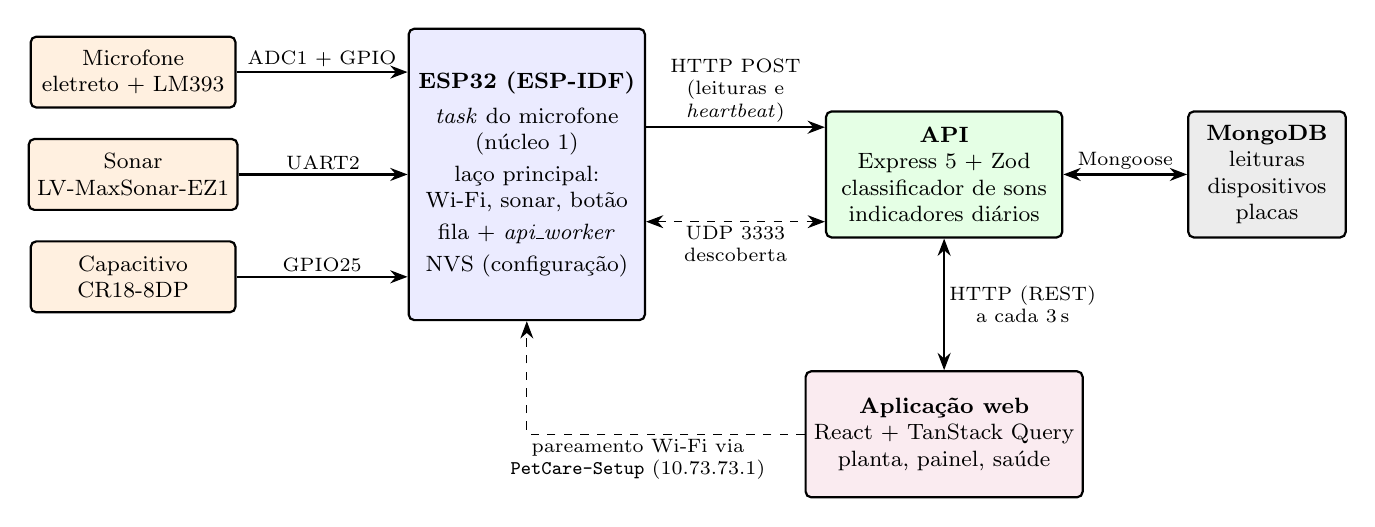
\begin{tikzpicture}[
  font=\footnotesize,
  >={Stealth[length=2.2mm]},
  bloco/.style={draw, rounded corners=2pt, thick, align=center, fill=white, inner sep=3pt},
  sensor/.style={bloco, fill=orange!12, minimum width=2.6cm, minimum height=0.9cm},
  esp/.style={bloco, fill=blue!8, minimum width=3.0cm, minimum height=3.7cm},
  srv/.style={bloco, fill=green!10, minimum width=3.0cm, minimum height=1.6cm},
  db/.style={bloco, fill=gray!15, minimum width=2.0cm, minimum height=1.6cm},
  rot/.style={font=\scriptsize, align=center, inner sep=1.5pt}
]
  % Sensores
  \node[sensor] (mic)   at (0, 1.3)  {Microfone\\eletreto + LM393};
  \node[sensor] (sonar) at (0, 0)    {Sonar\\LV-MaxSonar-EZ1};
  \node[sensor] (cap)   at (0, -1.3) {Capacitivo\\CR18-8DP};

  % ESP32
  \node[esp] (esp) at (5.0, 0) {\textbf{ESP32 (ESP-IDF)}\\[3pt]
     \textit{task} do microfone\\(núcleo 1)\\[2pt]
     laço principal:\\Wi-Fi, sonar, botão\\[2pt]
     fila + \textit{api\_worker}\\[2pt]
     NVS (configuração)};

  % API e banco
  \node[srv] (api) at (10.3, 0) {\textbf{API}\\Express 5 + Zod\\classificador de sons\\indicadores diários};
  \node[db]  (db)  at (14.4, 0) {\textbf{MongoDB}\\leituras\\dispositivos\\placas};

  % Web
  \node[srv, fill=purple!8] (web) at (10.3, -3.3) {\textbf{Aplicação web}\\React + TanStack Query\\planta, painel, saúde};

  % Sensores -> ESP32
  \draw[->, thick] (mic.east)   -- node[rot, above] {ADC1 + GPIO} (mic.east -| esp.west);
  \draw[->, thick] (sonar.east) -- node[rot, above] {UART2} (sonar.east -| esp.west);
  \draw[->, thick] (cap.east)   -- node[rot, above] {GPIO25} (cap.east -| esp.west);

  % ESP32 -> API
  \draw[->, thick] ([yshift=6mm]esp.east) -- node[rot, above] {HTTP POST\\(leituras e\\\textit{heartbeat})} ([yshift=6mm]esp.east -| api.west);
  \draw[<->, dashed] ([yshift=-6mm]esp.east) -- node[rot, below] {UDP 3333\\descoberta} ([yshift=-6mm]esp.east -| api.west);

  % API <-> MongoDB
  \draw[<->, thick] (api.east) -- node[rot, above] {Mongoose} (db.west);

  % Web <-> API
  \draw[<->, thick] (web.north) -- node[rot, right] {HTTP (REST)\\a cada 3\,s} (api.south);

  % Web -> ESP32 (pareamento)
  \draw[->, dashed] (web.west) -| node[rot, pos=0.3, below] {pareamento Wi-Fi via\\\texttt{PetCare-Setup} (10.73.73.1)} (esp.south);
\end{tikzpicture}
\caption{Arquitetura do PetCare. Setas contínuas: fluxo de dados em operação; tracejadas: fluxos de configuração (descoberta e pareamento).}
\label{fig:arquitetura}
\end{figure*}

\subsection{Contrato entre o ESP32 e a API}

O ponto central da integração é a rota \texttt{POST /api/readings}. O corpo é validado com Zod e aceita uma leitura ou um lote de até 100 leituras (objeto com o campo \texttt{readings} contendo um vetor). Os campos são: \texttt{sensorKey} (obrigatório), \texttt{value} (obrigatório), \texttt{recordedAt}, \texttt{durationMs} (até 60\,s), \texttt{kind}, \texttt{features} e \texttt{envelope} (até 128 valores entre 0 e 150). Exemplos de corpo enviados pelo firmware:

\begin{lstlisting}
{ "sensorKey": "esp32-01:proximity", "value": 1 }

{ "sensorKey": "esp32-01:mic", "value": 48.3,
  "durationMs": 920,
  "features": { "f0Hz": 610, "f0StartHz": 560,
    "f0EndHz": 650, "voicedRatio": 0.72,
    "zcr": 0.081, "bursts": 1 },
  "envelope": [31, 44, 48, 47, 40, 33] }
\end{lstlisting}

Os valores do segundo exemplo são ilustrativos do formato, e não uma medição. Quando a API tem a variável \texttt{DEVICE\_TOKEN} definida, a placa deve enviar o mesmo valor no cabeçalho \texttt{x-device-token}; caso contrário, a API responde 401. A API também atualiza o horário da última comunicação da placa, usado para mostrá-la como \textit{online} ou \textit{offline}; um dispositivo é considerado \textit{online} se enviou leitura nos últimos 5 minutos.

\subsection{API}

A API é organizada em módulos por domínio (\texttt{devices}, \texttt{readings}, \texttt{pairing}, \texttt{pets}, \texttt{insights}), cada um com modelo, esquemas de validação, rotas e serviço. Além da ingestão, ela oferece o cadastro dos itens da planta (nome, tipo, \textit{sensorKey}, posição em porcentagem da planta e capacidade do pote), o histórico por dispositivo, o estado calculado de cada item (último nível, eventos no dia, \textit{online}), a lista de placas pareadas e um servidor UDP que responde à descoberta.

\paragraph{Classificação das vocalizações.}
Quando a leitura do microfone não traz o tipo (\texttt{kind}), a API o estima por regras aplicadas em ordem (Tabela~\ref{tab:classificador}), inspiradas na literatura de acústica felina, que relaciona duração, $f_0$ e contorno de entonação dos miados ao contexto \citep{schotz2019}. Manter as regras na API permite ajustar os limiares sem regravar o firmware. \pendente{Os limiares não foram validados com gravações rotuladas; ver Seção~\ref{sec:resultados}.}

\begin{table}[!ht]
\caption{Regras do classificador de vocalizações, aplicadas em ordem (\texttt{vocalization.classifier.ts}).}
\label{tab:classificador}
\centering
\small
\begin{tblr}{
  colspec={X[0.9,l] X[2,l]},
  row{1}={font=\bfseries},
  hline{1,Z}={0.8pt}, hline{2}={0.4pt},
  rowsep=1pt
}
Tipo & Regra \\
Sibilo/rosnado & fração tonal $< 0{,}3$ e ZCR $\geq 0{,}25$; ou $f_0 < 250$\,Hz e duração $> 0{,}8$\,s \\
Tagarelar & $\geq 3$ rajadas com duração média por rajada $< 200$\,ms \\
Trinado & duração $< 0{,}6$\,s e $f_0$ subindo mais de 300\,Hz/s \\
Uivo & duração $\geq 1{,}5$\,s e (volume $\geq 50$ ou variação de $f_0 \geq 250$\,Hz); sem tom disponível, só a duração \\
Miado longo & duração $\geq 0{,}8$\,s \\
Miado curto & demais casos \\
\end{tblr}
\end{table}

\paragraph{Indicadores diários.}
O módulo \texttt{insights} agrega as leituras por dia: consumo de água e ração (quedas de nível de pelo menos 2 pontos percentuais, após suavização em janelas de 5 minutos, com subidas de 5 pontos ou mais tratadas como reabastecimento), número e duração das visitas à caixa de areia (permanências acima de 30 minutos são descartadas como falha de detecção) e vocalizações por tipo, inclusive noturnas (22h--6h). A aba de saúde compara esses valores com faixas de referência e com a própria linha de base do gato. Como o CR18-8DP só fornece 0\,\% ou 100\,\%, o cálculo de consumo, pensado para nível contínuo, fica restrito a transições cheio/vazio (Seção~\ref{sec:resultados}).

\subsection{Aplicação web}

A aplicação tem cinco páginas: \textbf{planta baixa} (itens arrastáveis sobre a planta da casa, com estado em tempo quase real), \textbf{painel} (gráficos por dispositivo, incluindo a forma de onda do envelope de cada som colorida pelo tipo detectado), \textbf{saúde} (consumo, caixa de areia e vocalizações, com perfil do gato), \textbf{dispositivos} (tabela de cadastro) e \textbf{configurações} (pareamento guiado da placa e lista de placas pareadas). Os dados são atualizados por consulta periódica a cada 3\,s. \pendente{Inserir capturas de tela da planta baixa, do painel e da aba de saúde.}

\section{Desenvolvimento}
\label{sec:desenvolvimento}

O código foi versionado com Git, com mensagens no padrão \textit{Conventional Commits} e integração por \textit{pull request}. A Tabela~\ref{tab:linhadotempo} resume a linha do tempo a partir do histórico do repositório. \pendente{Acrescentar as etapas de hardware que não aparecem no histórico: compra dos componentes, montagem, testes de bancada e troca do sensor de nível pelo CR18-8DP.}

\begin{table}[!ht]
\caption{Linha do tempo do desenvolvimento (histórico Git, 2026).}
\label{tab:linhadotempo}
\centering
\small
\begin{tabularx}{\linewidth}{l>{\hsize=1.000\hsize\raggedright\arraybackslash}X}
\toprule
\textbf{Data} & \textbf{Marco} \\
\midrule
12/11 & \textit{Commit} inicial: aplicação web, API e esboço do firmware em Arduino \\
16/11 & Firmware migrado para ESP-IDF: módulos de configuração (NVS), pareamento por ponto de acesso, descoberta UDP e leitura do sonar por UART \\
16/11 & API: módulo de pareamento de placas e servidor de descoberta UDP; web: página de configurações com pareamento guiado; documentação do ambiente ESP-IDF \\
16/11 & Correções: recuperação do Wi-Fi após quedas, escape de JSON, vazamento do \textit{token} do dispositivo e descoberta em Docker; integração do ramo \texttt{feature/wifi-and-sonar} (PR~\#1) \\
16/11 & Microfone: extração de características acústicas no firmware e classificação na API; aba de saúde; revisão visual da interface \\
17/11 & Gráfico da forma de onda (envelope) com os segmentos coloridos por tipo de som \\
22/11 & Monitor do sinal do microfone ao vivo (firmware, API e web); módulo \texttt{capacitive\_sensor} reescrito e publicado \\
22/11 & Assistente ``Adicionar dispositivo'' e portal cativo de configuração servido pela placa \\
22/11 & Reorganização da aplicação (Início com abas, página por sensor, Resumo) e correção da avaliação de saúde sem dados \\
\bottomrule
\end{tabularx}
\end{table}

\subsection{Problemas encontrados e correções}

Os \textit{commits} de correção registram três problemas relevantes:

\begin{itemize}
  \item \textbf{Wi-Fi que não se recuperava após quedas.} O tempo para abrir o ponto de acesso era contado a partir da inicialização, e não do início da queda; uma queda curta deixava a placa presa no modo de pareamento. A correção passou a contar o tempo desde o início da queda, a tentar a rede salva a cada 30\,s enquanto o ponto de acesso estiver ocioso e a fechá-lo quando a rede volta. Na mesma correção, a sub-rede do ponto de acesso foi movida para 10.73.73.0/24, para não colidir com redes domésticas em 192.168.4.0/22.
  \item \textbf{JSON malformado.} SSID e prefixo eram interpolados sem escape nos corpos JSON; um SSID com aspas quebraria a mensagem. Foi criado o módulo \texttt{json\_util}.
  \item \textbf{Vazamento do \textit{token} do dispositivo.} A rota \texttt{GET /api/pairing/config} devolvia o valor de \texttt{DEVICE\_TOKEN} ao navegador, anulando a proteção. Passou a informar apenas se o \textit{token} é exigido, e o usuário o digita na página de pareamento. Também foi corrigida a descoberta UDP (porta fixa 3333, independente da porta HTTP) e, em Docker, a API deixou de sugerir o IP interno da rede \textit{bridge}, que a placa não alcança.
\end{itemize}

\subsection{Ambiente de desenvolvimento do ESP32}

O firmware é compilado com o ESP-IDF 6.1.1 pela extensão oficial da Espressif no VS Code, a partir do WSL2 (Linux dentro do Windows). Esse arranjo trouxe dificuldades próprias:
\begin{itemize}
  \item o WSL2 não enxerga dispositivos USB. A placa (conversor USB-serial CH340) aparecia como COM3 no Windows, e foi preciso repassá-la ao Linux com o \texttt{usbipd-win}. O repasse se desfaz sempre que a placa reinicia ou o cabo é religado, e algumas leituras da porta serial travaram até o cabo ser reconectado;
  \item a rede do WSL2 é isolada por NAT: a placa, na rede de casa, não alcançava a API que rodava dentro do WSL. Foi necessário redirecionar a porta 3333 do Windows para o WSL (\texttt{netsh portproxy}) e liberá-la no firewall. A descoberta automática da API por \textit{broadcast} UDP não atravessa esse NAT, então o endereço da API passou a ser informado manualmente no pareamento;
  \item a tentativa de copiar a memória \textit{flash} da placa antes de regravá-la falhou com erro de dados corrompidos na leitura pela USB repassada. Como o código do sensor capacitivo só existia na placa, ele teve de ser reescrito. A lição registrada foi versionar todo código antes de gravá-lo.
\end{itemize}

\subsection{Problemas encontrados na integração com o protótipo}

\begin{itemize}
  \item \textbf{Microfone mudo.} O ADC estava saturado e, depois, o ajuste do comparador mostrou-se difícil (Seções~\ref{sec:mic-saturacao} e~\ref{sec:mic-regulagem}).
  \item \textbf{Eventos falsos do sonar.} Com o sensor a 17,8\,cm da superfície, a caixa de areia registrou mais de 80 ``visitas'' em uma manhã, alternando entrada e saída a cada poucos segundos, o que é compatível com a análise da Seção~\ref{sec:sonar}.
  \item \textbf{Pareamento com erro aparente.} A página indicava falha mesmo quando a placa tinha recebido a configuração, porque ela troca de rede logo depois de salvar e a resposta se perde. O endereço da API sugerido era o IP interno do WSL, inalcançável pela placa.
  \item \textbf{Erros de interface.} Duas classes do Tailwind v4 usadas como cor (\texttt{border-y-400} e \texttt{border-r-500}) são interpretadas como largura de borda e deformaram a tela; e a avaliação de saúde exibia ``Saudável'' sem dados (Seção~\ref{sec:arquitetura}).
\end{itemize}
\pendente{Acrescentar outros problemas de hardware vividos pela equipe (alimentação, mau contato, fixação dos sensores).}

\section{Resultados}
\label{sec:resultados}

Esta seção separa o que está evidenciado pelo código, pelo histórico e pelo registro serial do protótipo daquilo que ainda precisa ser medido. Nenhum resultado quantitativo de desempenho foi incluído antes dos testes.

\subsection{O que funcionou}

\begin{itemize}
  \item \textbf{Integração ponta a ponta}: firmware, API, banco e aplicação web foram integrados pelo contrato da Seção~\ref{sec:arquitetura}, e a stack completa sobe com Docker Compose.
  \item \textbf{Pareamento e rede}: no registro serial do protótipo, a placa abriu o ponto de acesso \texttt{PetCare-Setup} (10.73.73.1) após 10\,s sem conexão, como projetado. \pendente{Confirmar se o pareamento pela página de configurações e a descoberta UDP funcionaram na rede de teste.}
  \item \textbf{Sonar}: a leitura serial invertida pela UART2, sem inversor externo, produziu distâncias válidas; a linha de base foi calibrada (17,8\,cm no registro serial).
  \item \textbf{Robustez da comunicação}: as correções da Seção~\ref{sec:desenvolvimento} trataram a queda de Wi-Fi, o JSON malformado e o vazamento do \textit{token}.
  \item \textbf{Sensor capacitivo}: o CR18-8DP está ligado ao GPIO25 e é lido pelo firmware do protótipo. \pendente{Confirmar se as transições 0\,\%/100\,\% apareceram corretamente na aplicação.}
\end{itemize}

\subsection{O que não funcionou ou ficou limitado}

\begin{itemize}
  \item \textbf{Geometria do sonar}: com linha de base de 17,8\,cm e saturação do sensor em 15,24\,cm, a queda máxima possível ($\approx 2{,}5$\,cm) é menor que o limiar de entrada de 10\,cm (Seção~\ref{sec:sonar}). \pendente{Confirmar e registrar o teste após reposicionar o sensor.}
  \item \textbf{Nível dos potes}: a saída liga/desliga do CR18-8DP não fornece nível contínuo; o cálculo de consumo em ml/g da aba de saúde, pensado para nível em porcentagem, fica restrito a transições cheio/vazio. O código do módulo ainda não está no repositório.
  \item \textbf{Microfone}: o volume é apenas relativo, a resolução efetiva é limitada pela ausência de pré-amplificador e o ronronar não é detectado (Seção~\ref{sec:mic}).
  \item \textbf{Classificador}: as regras não foram validadas com gravações rotuladas, de modo que não há taxa de acerto conhecida.
  \item \textbf{Perda de eventos}: leituras geradas sem rede são descartadas (Seção~\ref{sec:firmware}).
\end{itemize}

\subsection{Testes a realizar}
\label{sec:testes}

\pendente{Preencher com os testes de bancada. Sugestões:}
\begin{enumerate}
  \item \pendente{Sonar: distância medida versus distância real (trena) em 5--10 pontos; número de entradas/saídas detectadas versus observadas em um período (verdadeiros e falsos positivos).}
  \item \pendente{Capacitivo: estado da saída com pote cheio, vazio e intermediário, com água e com ração; tensão no GPIO25 nos dois estados.}
  \item \pendente{Microfone: amplitude de AO no osciloscópio; detecção de sons a 0,5, 1 e 1,5\,m; matriz de confusão do classificador com sons rotulados manualmente.}
  \item \pendente{Sistema: latência entre o evento e a exibição na web; estabilidade da conexão em algumas horas de operação; consumo de corrente da placa.}
\end{enumerate}

\section{Conclusão e trabalhos futuros}
\label{sec:conclusao}

Este relatório apresentou o PetCare, um sistema de monitoramento da rotina de gatos que combina um ESP32, três sensores de baixo custo e uma aplicação web. Do ponto de vista de instrumentação, o trabalho mostrou como parte do condicionamento normalmente feito em \textit{hardware} pode ser deslocada para o firmware: remoção de nível DC, decimação, estimativa de $f_0$ por autocorrelação e detecção de eventos com limiar adaptativo no microfone; inversão de linha na UART e detecção com histerese no sonar. Também ficaram evidentes os limites dessa abordagem: sem pré-amplificador nem filtro \textit{anti-aliasing}, o microfone fornece apenas medidas relativas; a geometria de instalação do sonar precisa respeitar a distância mínima do sensor; e o sensor capacitivo industrial exige adaptação de nível e fornece apenas presença ou ausência. \pendente{Completar com as conclusões dos testes.}

Como trabalhos futuros, propõem-se:
\begin{itemize}
  \item adicionar ao microfone um estágio de pré-amplificação e um filtro passa-baixas \textit{anti-aliasing} antes do ADC;
  \item reposicionar o sonar e permitir calibrar seus limiares pela interface;
  \item publicar o módulo \texttt{capacitive\_sensor} e usar vários sensores em alturas diferentes (ou um sensor de nível contínuo) para estimar o consumo;
  \item validar o classificador de vocalizações com gravações rotuladas e avaliar técnicas baseadas em espectro (FFT);
  \item armazenar leituras na placa quando a rede estiver fora do ar e reenviá-las com horário sincronizado;
  \item substituir a consulta periódica da interface por \textit{Server-Sent Events} ou \textit{WebSocket}.
\end{itemize}


\begin{declarations}

\begin{acknowledgements}
\pendente{Agradecimentos (professor(a) da disciplina, laboratório, colegas).}
\end{acknowledgements}

\begin{funding}
\pendente{Informar se houve financiamento. Caso contrário: ``Este trabalho não recebeu financiamento específico''.}
\end{funding}

\begin{contributions}
\pendente{Descrever a contribuição de cada autor usando a Taxonomia CRediT (\href{https://credit.niso.org/}{https://credit.niso.org/}), por exemplo: A1 desenvolveu o firmware; A2 desenvolveu a API e a aplicação web; A3 montou e testou o hardware. Todos os autores leram e aprovaram o texto final.}
\end{contributions}

\begin{interests}
Os autores declaram que não têm nenhum conflito de interesses. \pendente{Confirmar.}
\end{interests}

\begin{materials}
O código-fonte do firmware, da API e da aplicação web está disponível em \pendente{URL do repositório, se público; caso contrário, ``será disponibilizado mediante solicitação''}.
\end{materials}

\begin{aitools}
\pendente{Declarar o uso de ferramentas de IA generativa. O histórico do repositório registra commits coassinados por um assistente de IA (Claude), e este rascunho de relatório também foi gerado com auxílio de IA; descrever onde foram empregadas (código, textos, revisão) e as versões.}
\end{aitools}

\begin{furtherinformation}
Os testes envolvem a observação de animais domésticos dos próprios autores, sem procedimentos invasivos. \pendente{Confirmar e ajustar.}
\end{furtherinformation}

\end{declarations}

\bibliographystyle{apalike-sol}
\bibliography{refs}

\clearpage
\appendix
% Apêndice: telas da aplicação web (capturas do protótipo em funcionamento).
% As imagens estão em figuras/telas/. Os dados exibidos são do protótipo real;
% \pendente marca as capturas que devem ser refeitas depois da remontagem do sonar.

\section{Telas da aplicação}\label{sec:apendice-telas}

Esta seção reúne capturas da aplicação web em funcionamento com o protótipo. A navegação
tem três áreas principais (Início, Resumo e Saúde do gato) e uma página por sensor, aberta ao
tocar em qualquer cartão, marcador da planta ou evento da linha do tempo.

\pendente{Refazer as capturas da caixa de areia depois de remontar o sonar: os números de
visitas exibidos vêm de disparos falsos do sensor montado a 17,8~cm da superfície
(ver Seção~\ref{sec:resultados}).}

\begin{figure}[htbp]
  \centering
  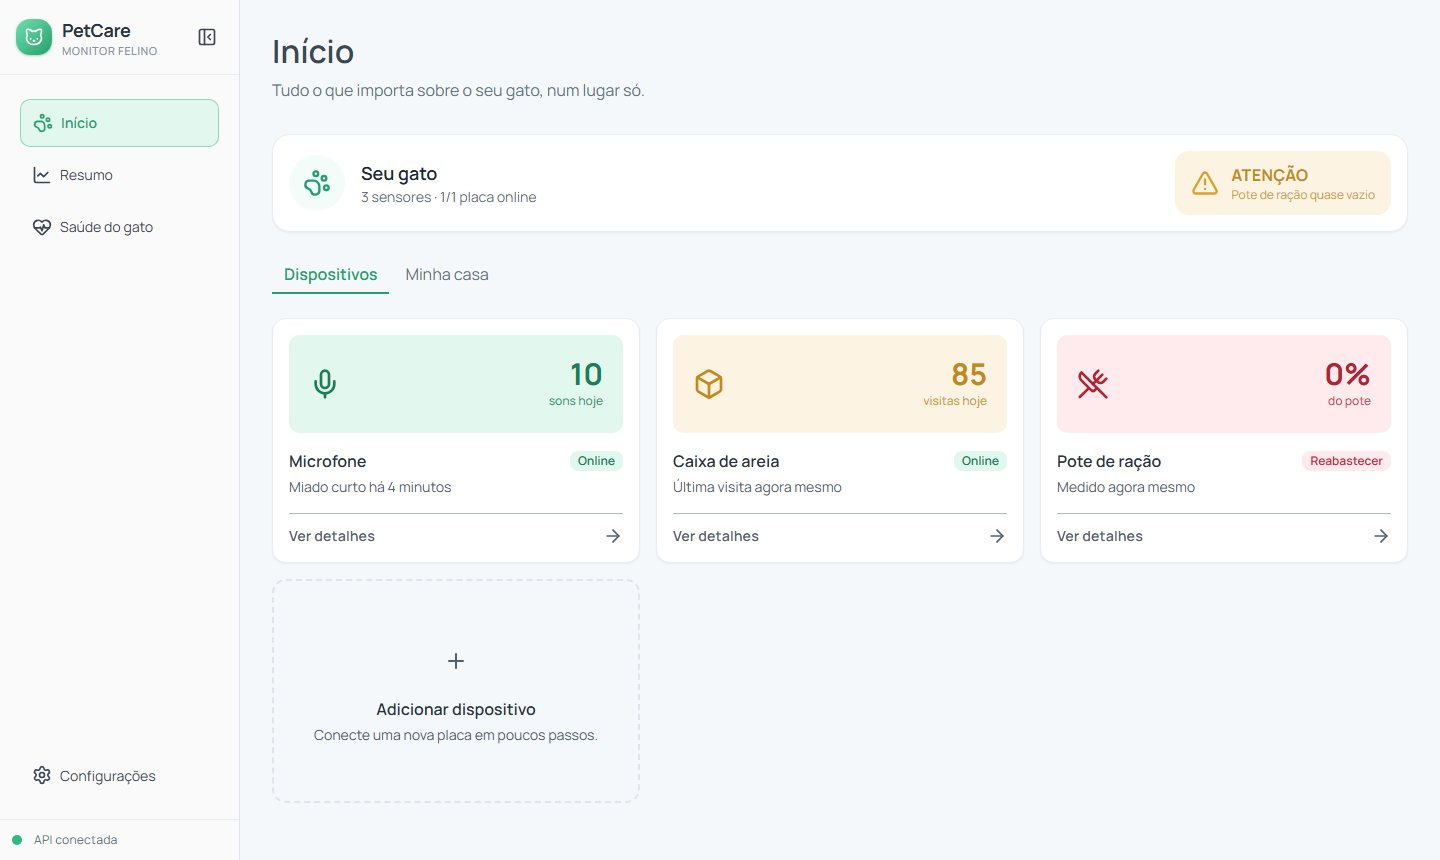
\includegraphics[width=\linewidth]{figuras/telas/inicio-dispositivos.jpg}
  \caption{Início, aba \emph{Dispositivos}: selo de estado geral da casa e um cartão por
  sensor com o valor principal do dia.}
  \label{fig:tela-inicio-dispositivos}
\end{figure}

\begin{figure}[htbp]
  \centering
  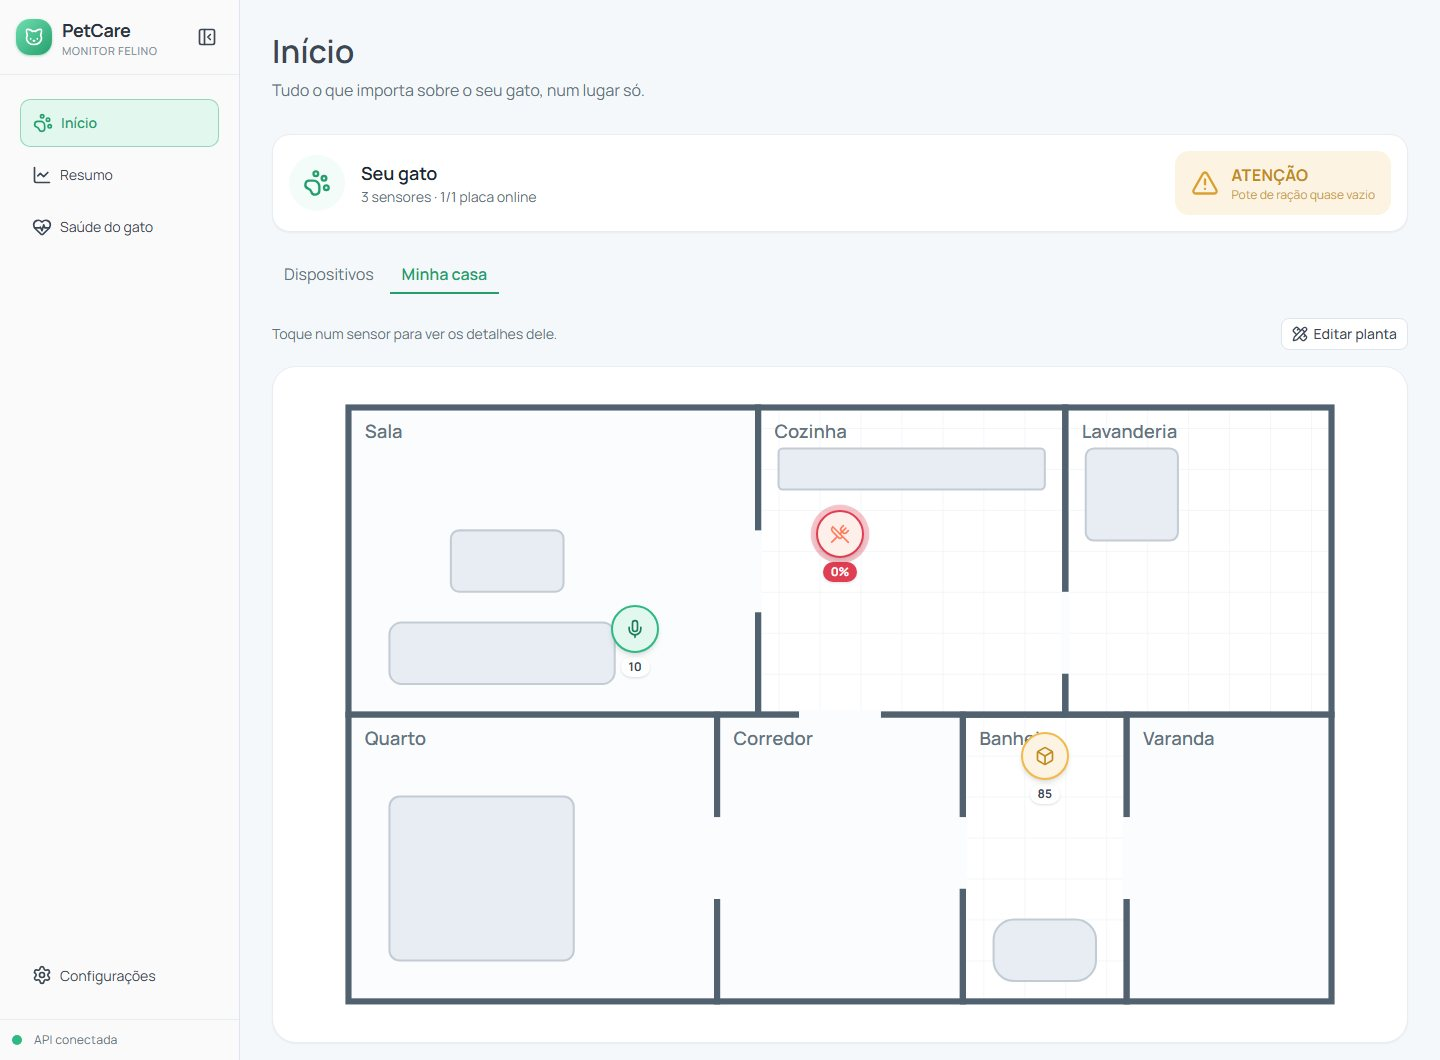
\includegraphics[width=\linewidth]{figuras/telas/inicio-casa.jpg}
  \caption{Início, aba \emph{Minha casa}: planta baixa com a posição de cada sensor.
  No modo de edição os sensores podem ser arrastados.}
  \label{fig:tela-inicio-casa}
\end{figure}

\begin{figure}[htbp]
  \centering
  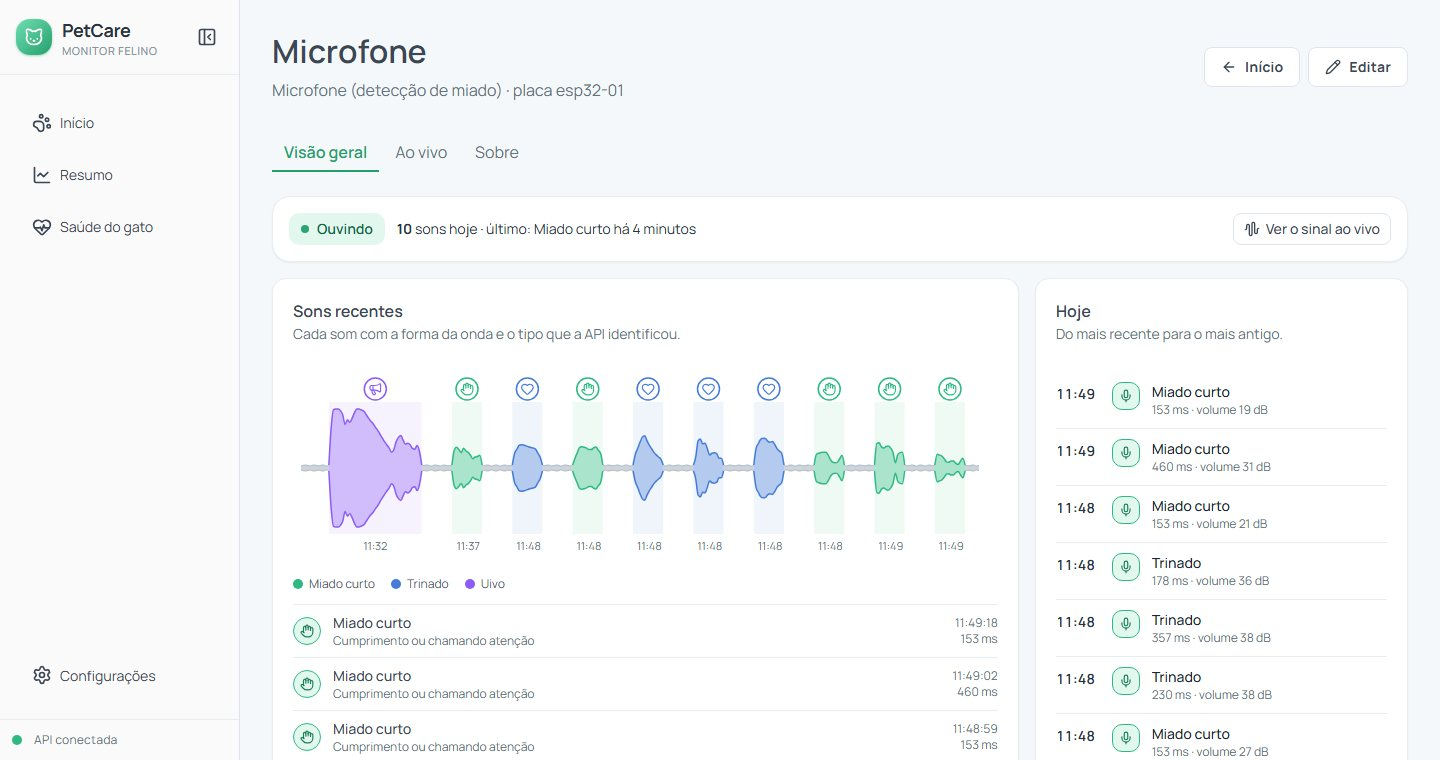
\includegraphics[width=\linewidth]{figuras/telas/sensor-microfone.jpg}
  \caption{Página do microfone, aba \emph{Visão geral}: sons recentes com a forma de onda
  (envelope de volume) e o tipo de vocalização classificado pela API.}
  \label{fig:tela-microfone}
\end{figure}

\begin{figure}[htbp]
  \centering
  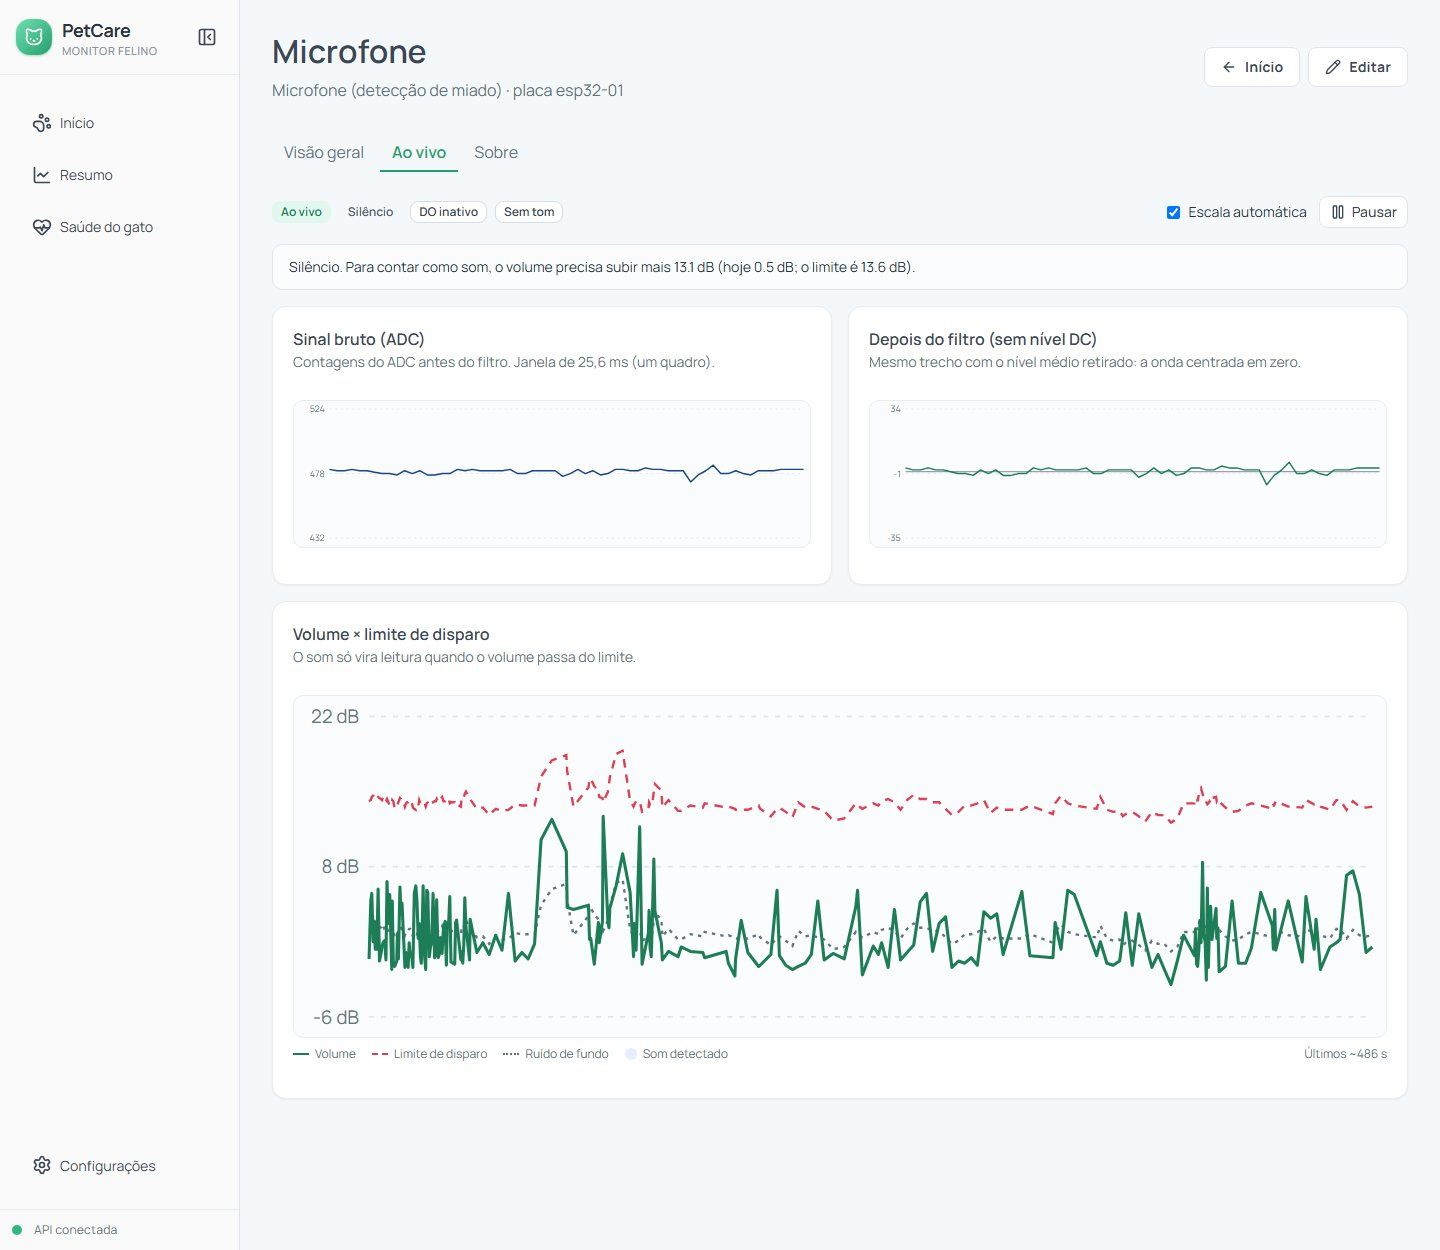
\includegraphics[width=\linewidth]{figuras/telas/sensor-microfone-ao-vivo.jpg}
  \caption{Página do microfone, aba \emph{Ao vivo}: sinal bruto do ADC, sinal após a remoção
  do nível DC e volume em relação ao limite de disparo, com diagnóstico automático.}
  \label{fig:tela-microfone-ao-vivo}
\end{figure}

\begin{figure}[htbp]
  \centering
  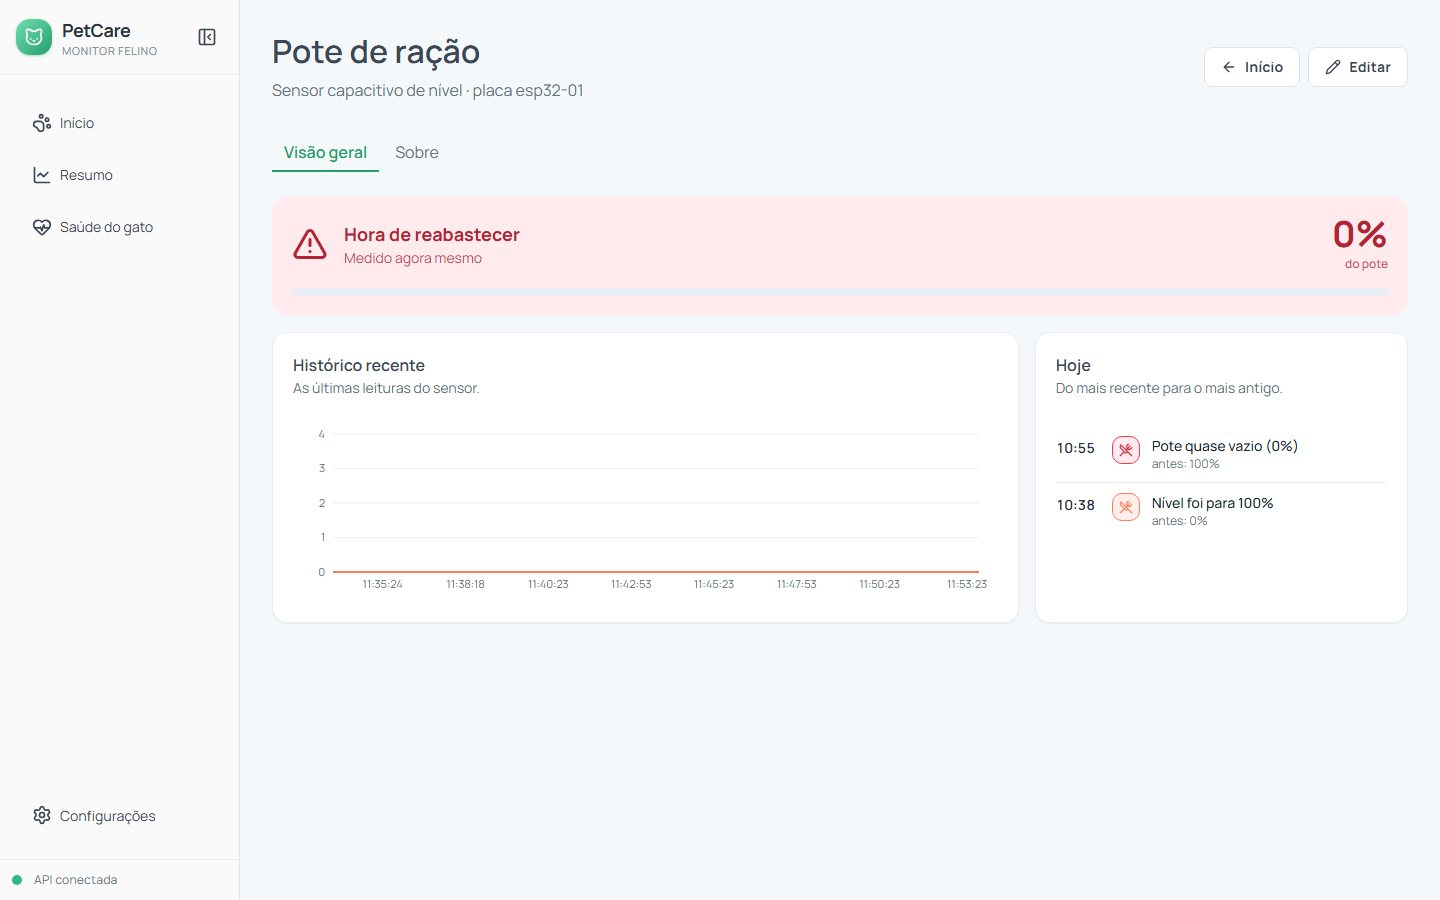
\includegraphics[width=\linewidth]{figuras/telas/sensor-pote.jpg}
  \caption{Página do pote de ração: estado atual, acontecimentos do dia e histórico das
  leituras do sensor capacitivo.}
  \label{fig:tela-pote}
\end{figure}

\begin{figure}[htbp]
  \centering
  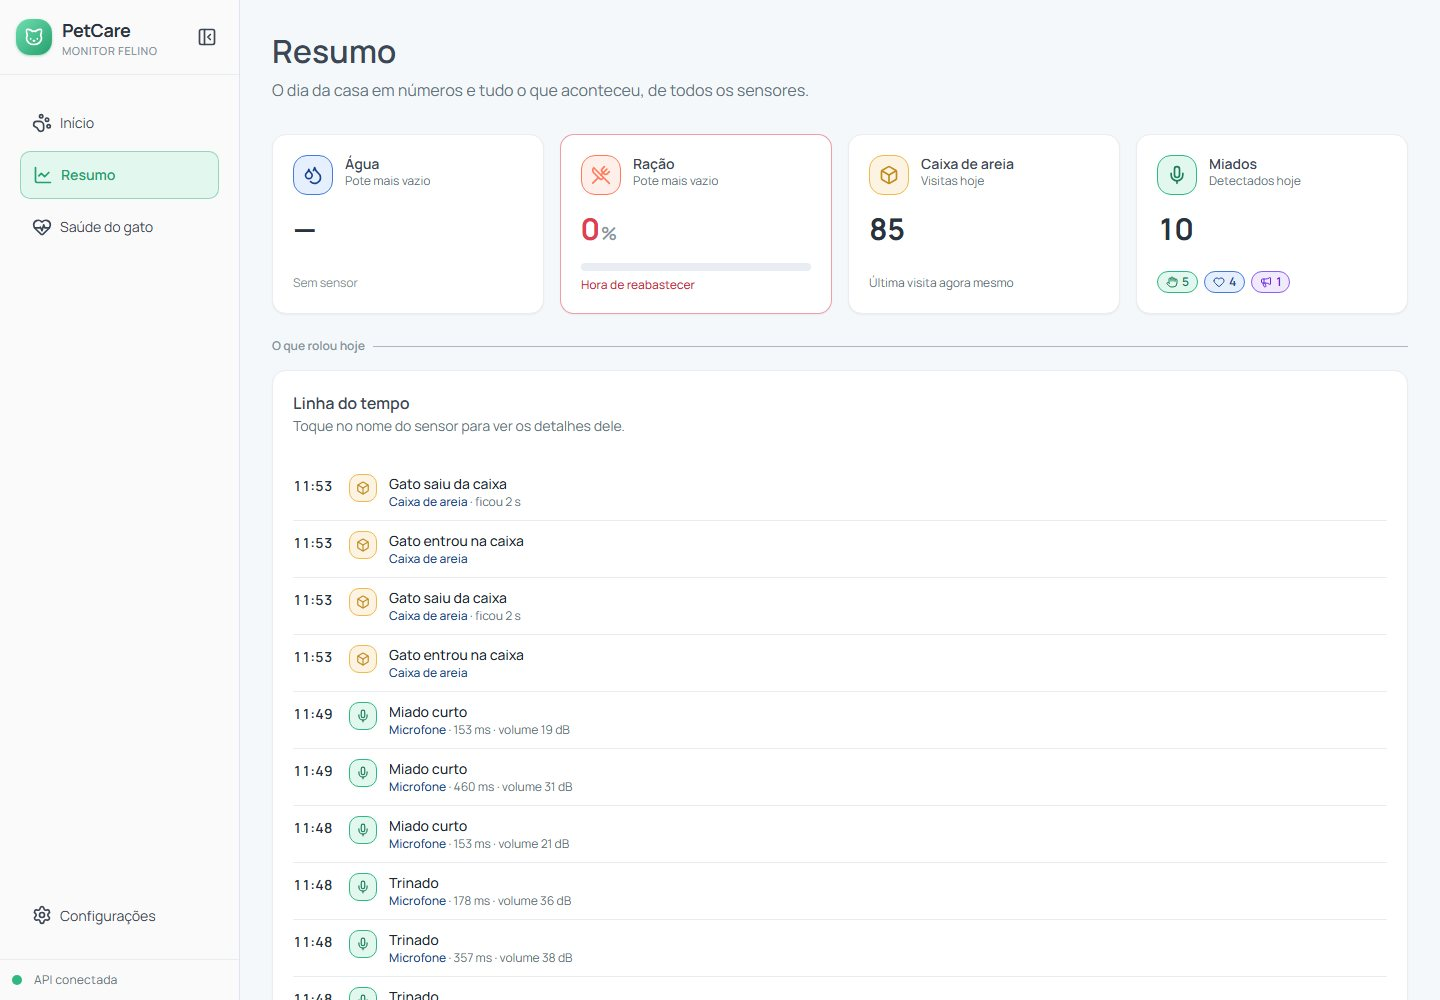
\includegraphics[width=\linewidth]{figuras/telas/resumo.jpg}
  \caption{Resumo: números do dia e linha do tempo com os acontecimentos de todos os sensores.}
  \label{fig:tela-resumo}
\end{figure}

\begin{figure}[htbp]
  \centering
  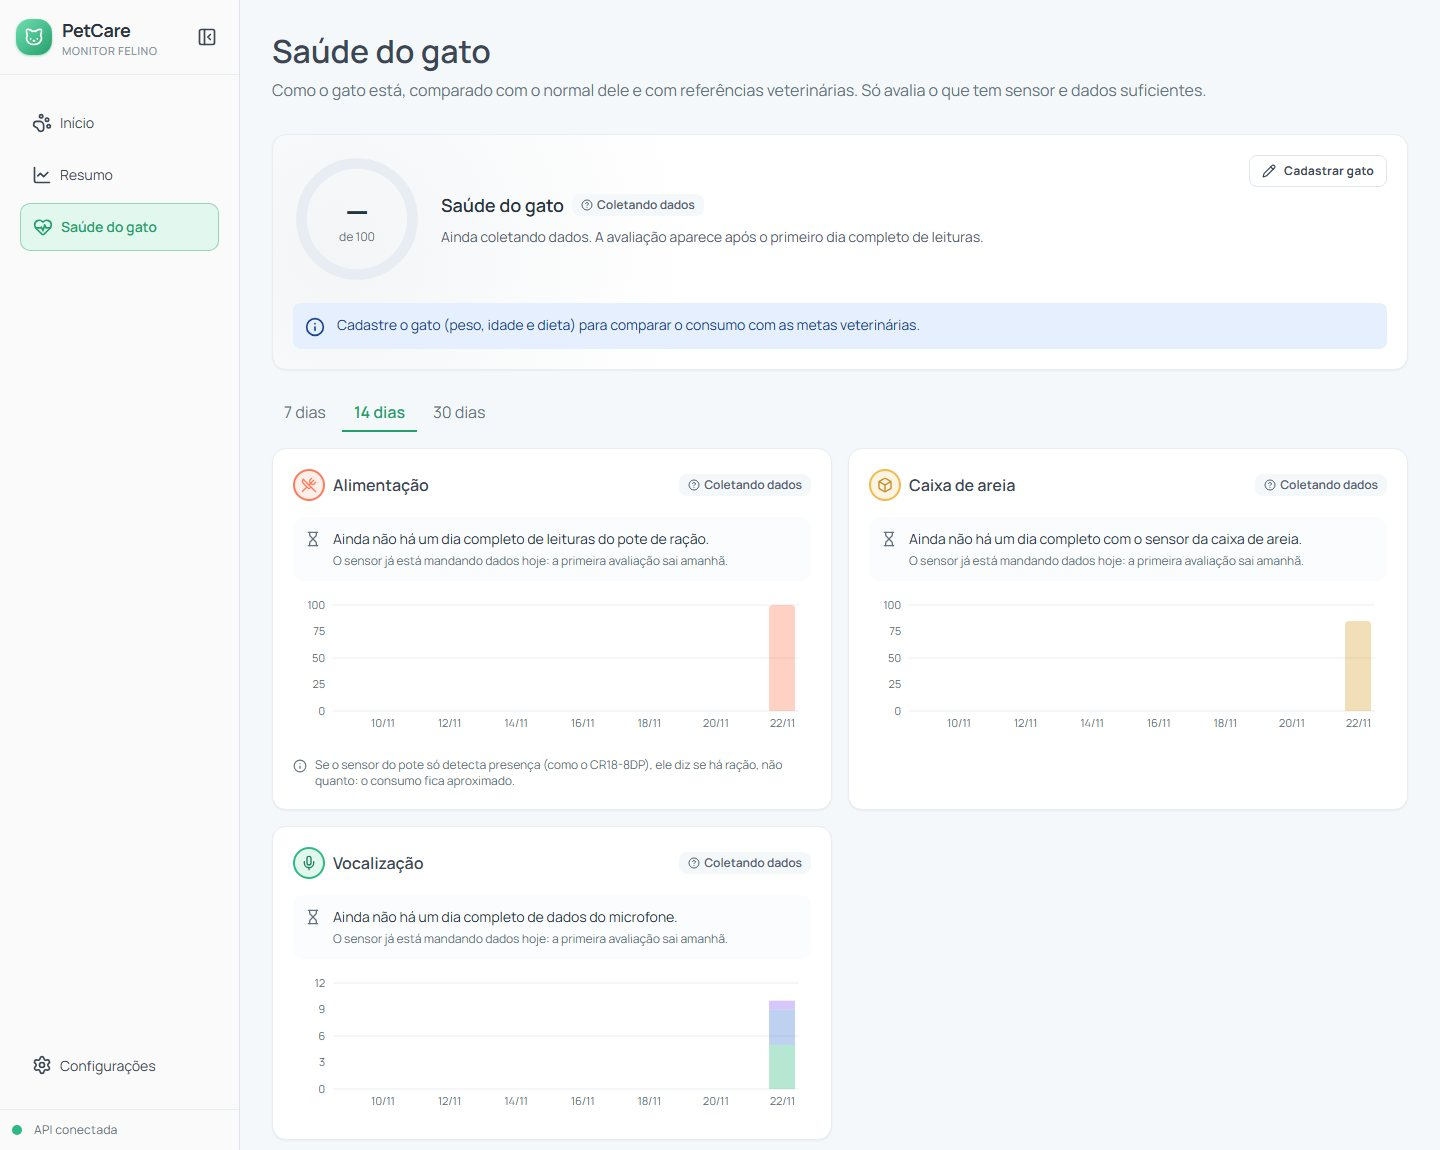
\includegraphics[width=\linewidth]{figuras/telas/saude.jpg}
  \caption{Saúde do gato: avaliação por área a partir dos dados diários. Sem dias completos
  de leitura, a aplicação indica ``Coletando dados'' em vez de um diagnóstico.}
  \label{fig:tela-saude}
\end{figure}

\begin{figure}[htbp]
  \centering
  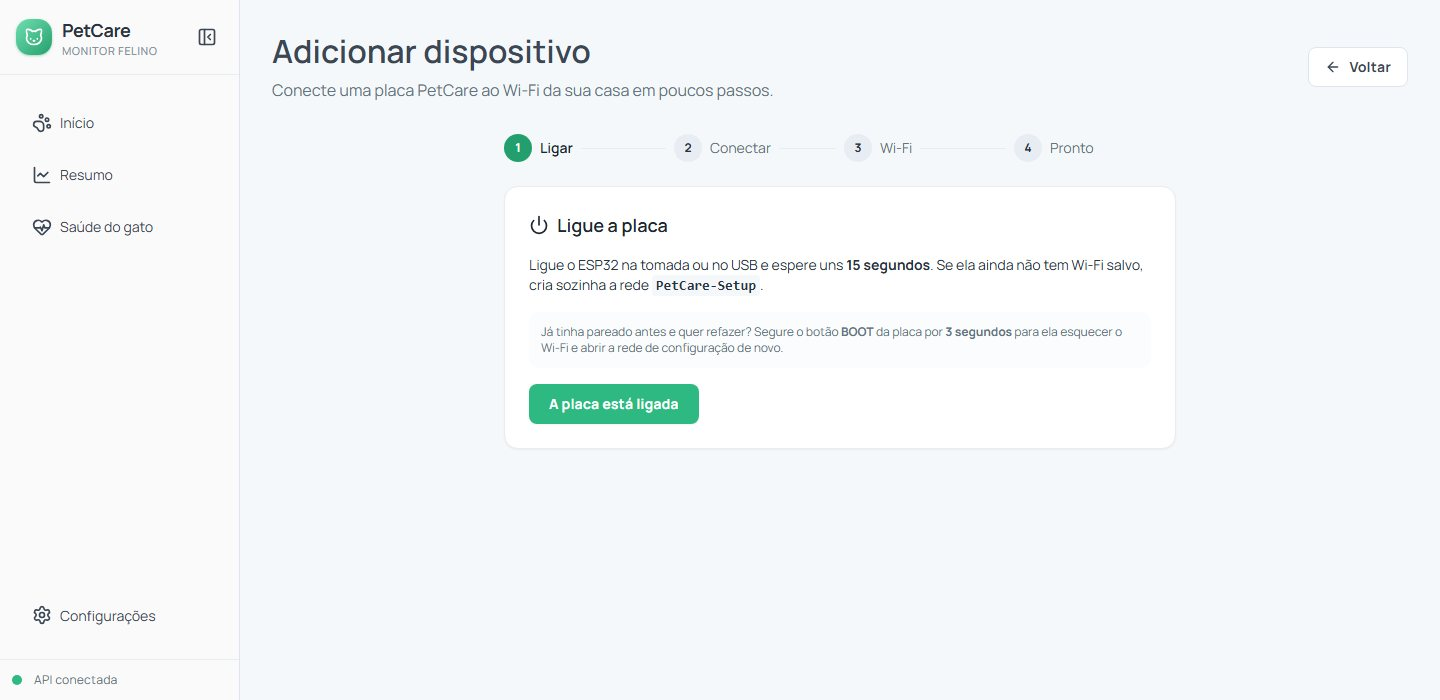
\includegraphics[width=\linewidth]{figuras/telas/adicionar-dispositivo.jpg}
  \caption{Assistente de pareamento de uma nova placa pela rede \texttt{PetCare-Setup}.}
  \label{fig:tela-adicionar}
\end{figure}


\end{document}
